\documentclass{article}
\usepackage[utf8]{inputenc}
\usepackage{graphicx}
\usepackage{wasysym}
\author{Felix Bello, Gilles Brunner}
\title{Arbeitsauftrag 2}
\begin{document}
	\maketitle
	\section{Einführung}
	\begin{itemize}
		\item[\Square] Linux
		\item[\Square] Apache
		\item[\Square] MariaDB
		\item[\Square] PHP
	\end{itemize}
	\section{LAMP}
	\textit{lucy:/home/gilles\# screen -S newScreen}
	\newline
	\textit{lucy:/home/gilles\# apt-get install mariadb-client-10.0 mariadb-server-10.0 apache2 apache2-doc php5 php5-mysql libapache 2-mod-php5}
	\newline
	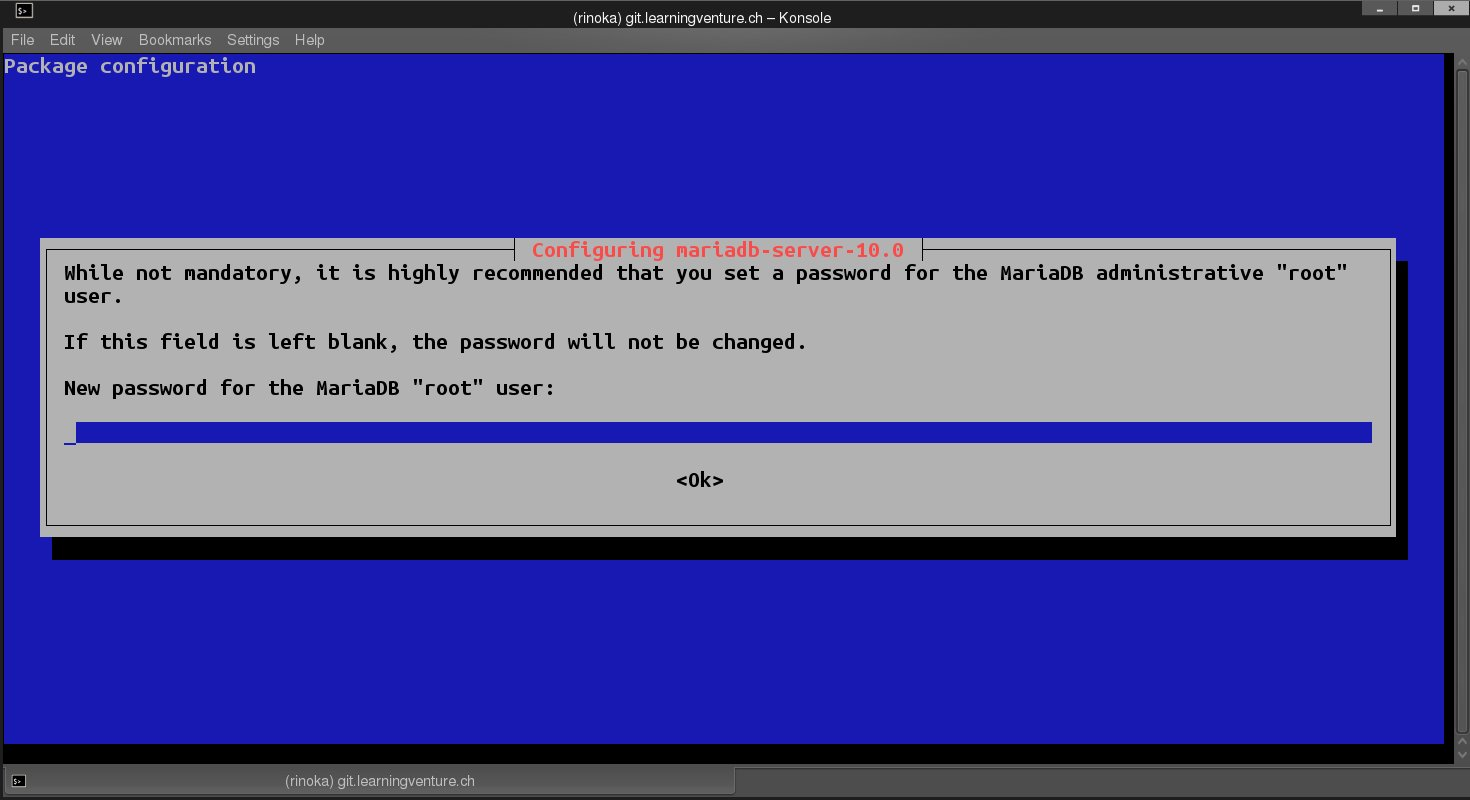
\includegraphics[width=13cm]{../Pics/3-lamp-stack-mariadb}
	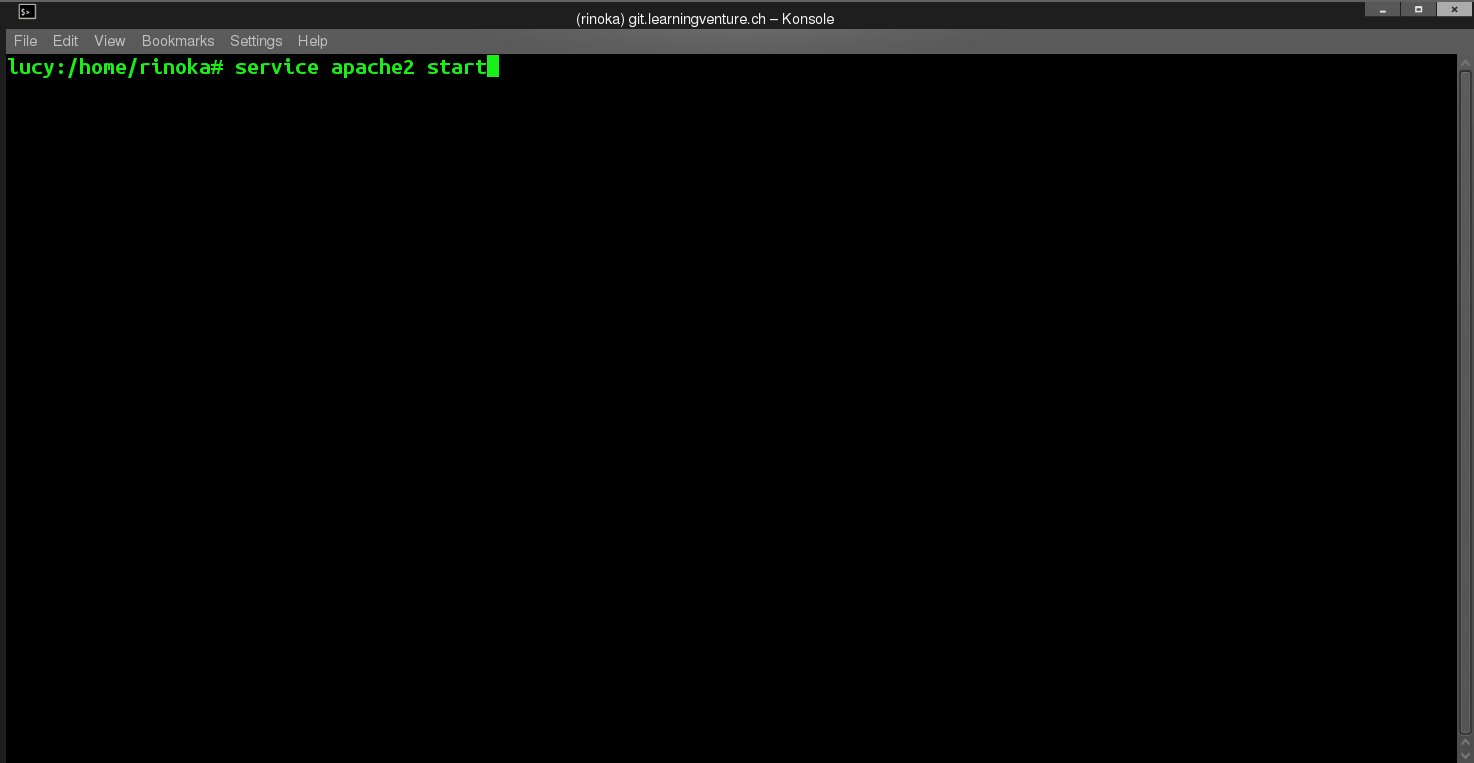
\includegraphics[width=13cm]{../Pics/start_apache}
	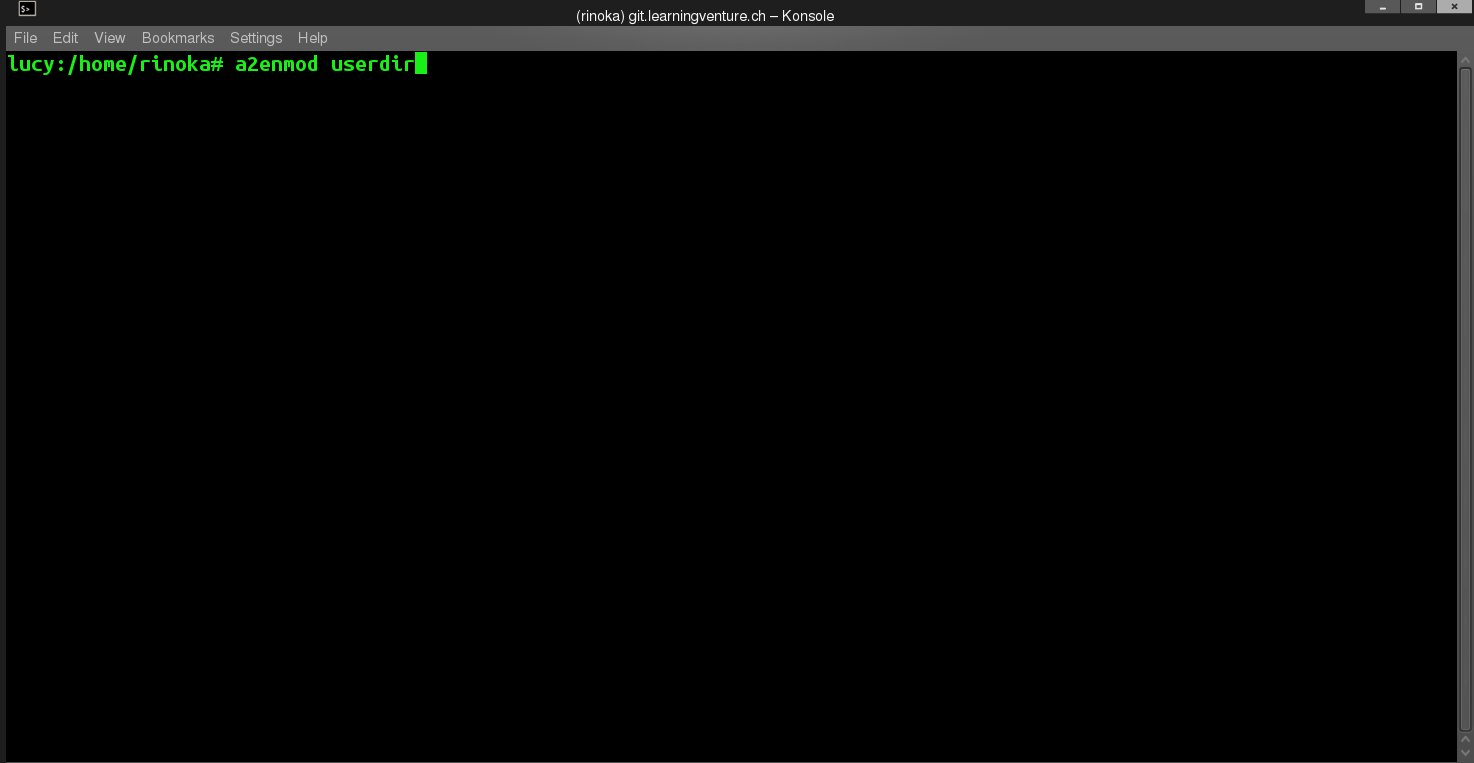
\includegraphics[width=13cm]{../Pics/a2enmod_userdir}
	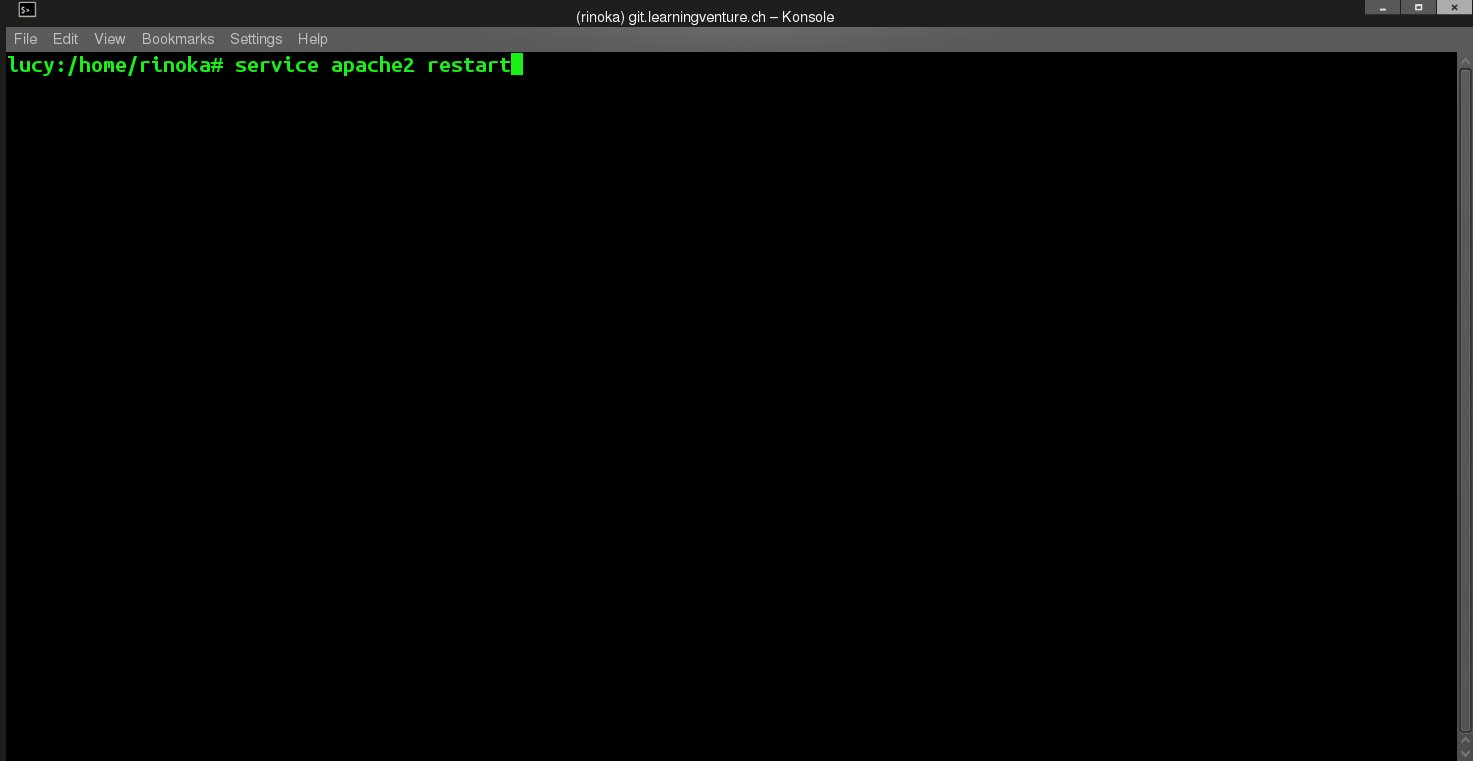
\includegraphics[width=13cm]{../Pics/apach2restart}
	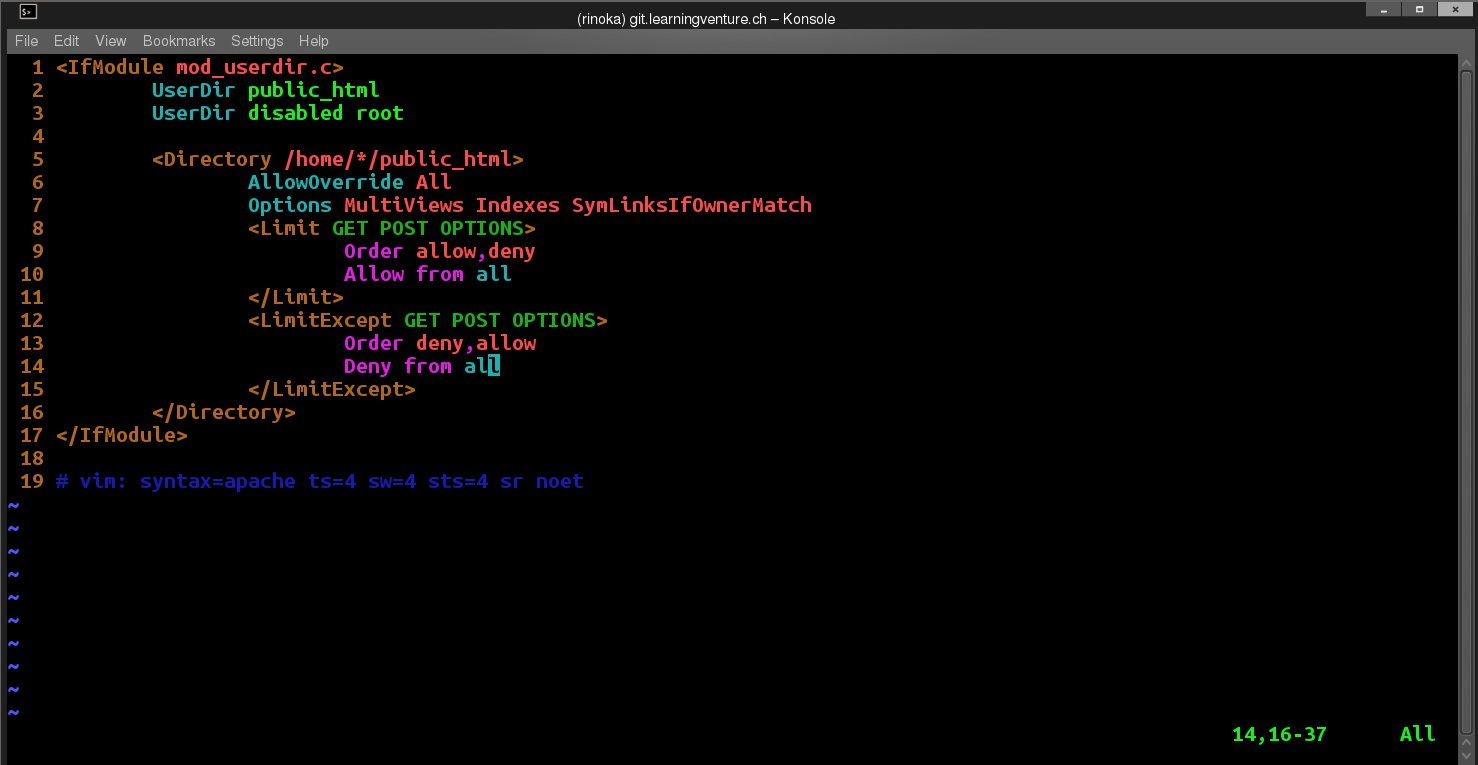
\includegraphics[width=13cm]{../Pics/6_userdirconf}
	\subsection{Linux}
	\subsection{Apache}
	\subsection{MariaDB}
	\subsection{PHP}
	\section{WordPress}
	\section{OwnCloud}
\end{document}